\documentclass{beamer}
%\documentclass[handout]{beamer}

\mode<presentation>
{
  %\usetheme{CambridgeUS}
  %\usetheme{Frankfurt}
  \usetheme{Singapore}
  %\usecolortheme{crane}
  \usefonttheme{professionalfonts}
  %\usefonttheme[onlymath]{serif}
  
  \setbeamertemplate{blocks}[rounded][shadow=true]
}

\usepackage{pgfpages}

\usepackage{alltt,verbatim,amsmath,times}
\usepackage{bm}
\usepackage[english]{babel}
\usepackage[utf8]{inputenc}

%\usepackage{times}
%\usepackage[T1]{fontenc}
% Or whatever. Note that the encoding and the font should match. If T1
% does not look nice, try deleting the line with the fontenc.

%\usepackage{hyperref}

\usepackage{pdfanim}
\usepackage{multimedia,xmpmulti}

\PDFAnimLoad[width=\textwidth,loop,interval=40]{exp3a}{exp3a/pic}{310}%

\definecolor{dark red}{HTML}{E41A1C}
\definecolor{dark green}{HTML}{4DAF4A}
\definecolor{dark violet}{HTML}{984EA3}
\definecolor{dark blue}{HTML}{084594}
\definecolor{dark orange}{HTML}{FF7F00}
\definecolor{light blue}{HTML}{377EB8}
\definecolor{light red}{HTML}{FB9A99}
\definecolor{light violet}{HTML}{CAB2D6}

\setbeamercolor{boxed}{fg=black,bg=uaf yellow}

\newcommand{\CC}{\mathbb{C}}
\newcommand{\NN}{\mathbb{N}}
\newcommand{\RR}{\mathbb{R}}
\newcommand{\ZZ}{\mathbb{Z}}
\newcommand{\Acal}{\mathcal{A}}
\newcommand{\Bcal}{\mathcal{B}}
\newcommand{\Ccal}{\mathcal{C}}
\newcommand{\Ncal}{\mathcal{N}}
\newcommand{\Kcal}{\mathcal{K}}

\newcommand{\bF}{\mathbf{F}}
\newcommand{\bQ}{\mathbf{Q}}
\newcommand{\bU}{\mathbf{U}}
\newcommand{\bbU}{\bar{\bU}}
\newcommand{\bu}{\mathbf{u}}
\newcommand{\bv}{\mathbf{v}}
\newcommand{\bx}{\mathbf{x}}

\newcommand{\Div}{\nabla\cdot}
\newcommand{\eps}{\epsilon}
\newcommand{\grad}{\nabla}
\newcommand{\lap}{\triangle}
\DeclareMathOperator{\trace}{tr}
\renewcommand{\bar}{\overline}

\newcommand{\ddx}[1]{\frac{\partial #1}{\partial x}}
\newcommand{\ddy}[1]{\frac{\partial #1}{\partial y}}
\newcommand{\pp}[2]{\frac{\partial #1}{\partial #2}}
\newcommand{\ppt}[1]{\frac{\partial #1}{\partial t}}
\newcommand{\ppT}[1]{\frac{\partial #1}{\partial T}}
\newcommand{\ppx}[1]{\frac{\partial #1}{\partial x}}
\newcommand{\ppy}[1]{\frac{\partial #1}{\partial y}}
\newcommand{\ppz}[1]{\frac{\partial #1}{\partial z}}
\newcommand{\ppxx}[1]{\frac{\partial^2 #1}{\partial x^2}}
\newcommand{\ppzz}[1]{\frac{\partial^2 #1}{\partial z^2}}

%\setbeamercolor{redtext}{fg=red!80!black}
\setbeamercolor{redtext}{fg=red!94!black}
%\setbeamercolor{greentext}{fg=green!80!black}
\setbeamercolor{greentext}{fg=green!60!black}
%\setbeamercolor{bluetext}{fg=blue!70!black}
\setbeamercolor{bluetext}{fg=blue!90!black}
\setbeamercolor{yellowtext}{fg=yellow!95!black}
\setbeamercolor{orangetext}{fg=yellow!50!red}

\newcommand{\green}{\usebeamercolor[fg]{greentext}}
\newcommand{\blue}{\usebeamercolor[fg]{bluetext}}
\newcommand{\red}{\usebeamercolor[fg]{redtext}}

\renewcommand{\L}{\emph{Left}}
\newcommand{\R}{\emph{Right}}



\title[weak and shallow ice sheet flows]{Weak and shallow: \\ New thinking about simulations of ice sheet flows}

\author[Bueler]{Ed Bueler}

\institute[UAF]{
  \tiny Dept of Mathematics and Statistics, and Geophysical Institute,
  University of Alaska Fairbanks
}

\date{\tiny 27 October, 2012}


\setbeamerfont{date}{size=\scriptsize}

\subject{ice sheet modelling, ice sheets, ice streams, numerical analysis, variational inequality}


%\begin{comment}
\AtBeginSection[]
{
  \begin{frame}<beamer>
    \frametitle{Outline}
    \tableofcontents[currentsection,hideallsubsections]
  \end{frame}
}
%\end{comment}


\begin{document}
\graphicspath{{figs/},{../commonfigs/},{photos/}}

\begin{frame}
  \titlepage
  \begin{center}
  \tiny supported by NASA grant NNX09AJ38C
  \end{center}
\end{frame}


\begin{frame}
  \frametitle{weak, shallow, and fairly new}

\begin{itemize}
\small
\item C.~Schoof (\textbf{2006}) \emph{A variational approach to ice stream flow}, J.~Fluid Mech.~556, 227--251
\medskip
\item E.~Bueler, J.~Brown (\textbf{2009}) \emph{Shallow shelf approximation as a “sliding law” in a thermodynamically coupled ice sheet model}, J.~Geophys.~Res.~114, F03008
\medskip
\item \alert<2>{G.~Jouvet}, E.~Bueler (\textbf{2012}) \emph{Steady, shallow ice sheets as obstacle problems: well-posedness and finite element approximation}, SIAM J.~Appl.~Math.~72 (4), 1292--1314
\medskip
\item \alert<2>{G.~Jouvet}, E.~Bueler, C.~Gr\"aser, R.~Kornhuber (\textbf{to appear})  \emph{A nonsmooth Newton multigrid method for a hybrid, shallow model of marine ice sheets}, Proc.~8th ICSCA, AMS Cont.~Math.
\end{itemize}

\small
\onslide<2>{\alert{G.~Jouvet} = Guillaume Jouvet, Free University of Berlin}
\end{frame}


% NO OUTLINE BECAUSE ONE APPEARS AT START OF EACH SECTION:
%\begin{comment}
\begin{frame}
  \frametitle{Outline}
  \tableofcontents[hideallsubsections]
  % You might wish to add the option [pausesections]
\end{frame}
%\end{comment}


\section[intro]{ice sheet flow: an introduction for non-glaciologists}


\begin{frame}{ice in glaciers is a viscous fluid}
\begin{columns}
\begin{column}{0.65\textwidth}
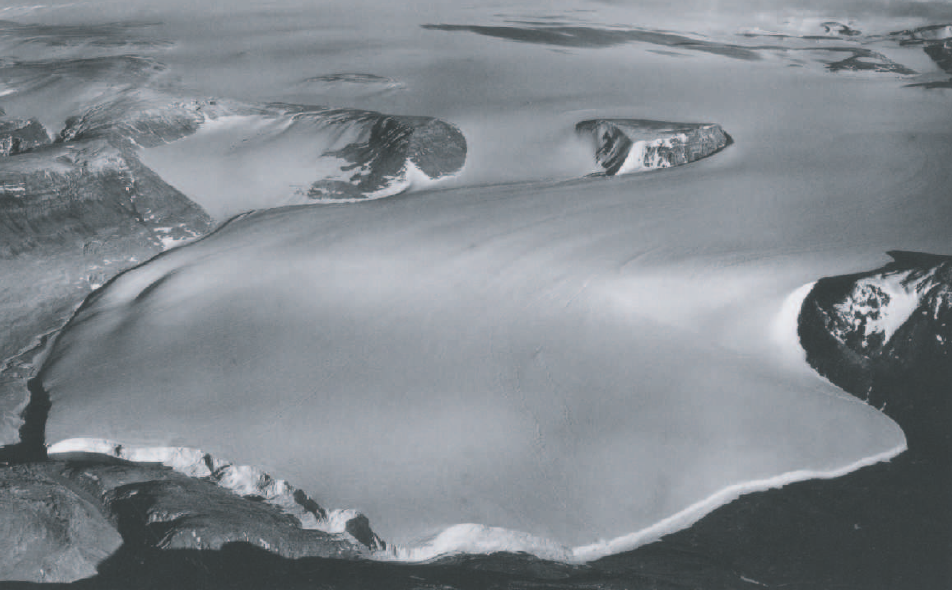
\includegraphics[width=1.0\textwidth]{polaris}
\end{column}
\begin{column}{0.35\textwidth}
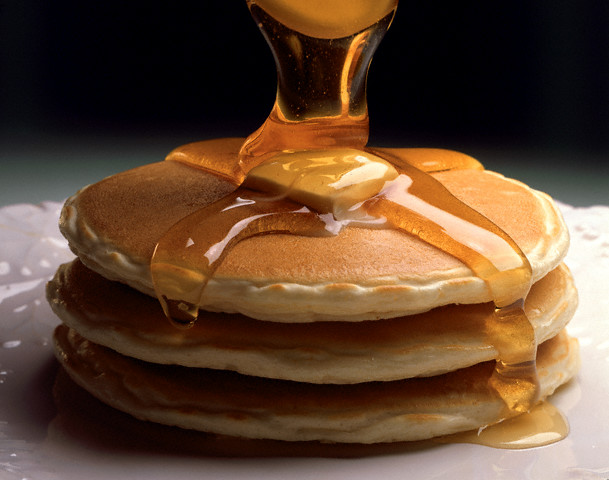
\includegraphics[width=1.0\textwidth]{pancakes}
\end{column}
\end{columns}

\bigskip\bigskip
\begin{itemize}
\item \dots at least: glaciers are viscous flows at the big scale
\item \emph{usage}: ``ice sheets'' are big, shallow glaciers
\end{itemize}
\end{frame}


\begin{frame}{ice in glaciers is a viscous fluid}

\begin{itemize}
\item primary variables: velocity $\mathbf{u}(\bx,t)$ and pressure $p(\bx,t)$
\item also: $\rho$ is density, $\mathbf{g}$ is gravity, $\nu$ is viscosity
\item if the glacier fluid were ``typical'' like liquid water we would model with Navier-Stokes equations:
\begin{align*}
\nabla \cdot \mathbf{u} &= 0 &&\text{\emph{incompressibility}} \\
\rho \left(\mathbf{u}_t + \mathbf{u}\cdot\nabla \mathbf{u}\right) &= -\nabla p + \nu \nabla^2 \mathbf{u} + \rho \mathbf{g} &&\text{\emph{stress balance}}
\end{align*}
\item but it is not typical!
\item e.g.~not addressed in ice sheet flow models:
  \begin{itemize}
  \item[$\circ$] turbulence
  \item[$\circ$] convection
  \item[$\circ$] coriolis force
  \item[$\circ$] density-driven flow
  \end{itemize}
\end{itemize}
\end{frame}


\begin{frame}{ice is a slow, shear-thinning viscous fluid}

\begin{itemize}
\item our glacier fluid is
  \begin{enumerate}
  \item ``slow'':
    $$\rho \left(\mathbf{u}_t + \mathbf{u}\cdot\nabla \mathbf{u}\right) \approx 0 \qquad \iff \qquad \begin{pmatrix} \text{forces of inertia} \\ \text{are negligible} \end{pmatrix}$$
  \item non-Newtonian (shear-thinning):
    $$\text{viscosity $\nu$ is not constant}$$
  \end{enumerate}
\end{itemize}
\end{frame}


\begin{frame}{ice is a slow, shear-thinning viscous fluid}

\begin{itemize}
\item notation: $\tau_{ij}$ is deviatoric stress tensor, $\mathbf{D}u_{ij}$ is strain rate tensor
\item the standard ice flow model is Glen-law Stokes:
\begin{align*}
\nabla \cdot \mathbf{u} &= 0 &&\text{\emph{incompressibility}} \\
0 &= - \nabla p + \nabla \cdot \tau_{ij} + \rho \mathbf{g} &&\text{\emph{slow stress balance}} \\
\mathbf{D}u_{ij} &= A \tau^{n-1} \tau_{ij} &&\text{\emph{Glen flow law}}
\end{align*}
\item $1.8 < n < 4.0$ ?  \quad when in doubt: $n=3$
\end{itemize}
\end{frame}


\begin{frame}{because ice is a slow fluid \dots}

\begin{itemize}
\item it is a time-independent Stokes problem:
  \begin{quote}
  \alert{geometry, boundary stress, and viscosity determine velocity field and pressure instantaneously} (in the model)
  \end{quote}
\item so: a time-stepping ice sheet code recomputes the velocity field at every time step, without requiring velocity from the previous step\footnote{to be a weatherman you've got to know which way the wind blows \dots but don't expect that much from a glaciologist}
\end{itemize}
\end{frame}


\begin{frame}{yes, ice sheets are ``shallow''}

\begin{itemize}
\item consider cross section of Greenland ice sheet at $71^\circ$ N
\small
  \begin{itemize}
  \item[$\circ$] {\color{dark green}{green}} and {\color{dark blue}{blue}}: usual vertically-exaggerated version
  \end{itemize}
  \begin{center}
    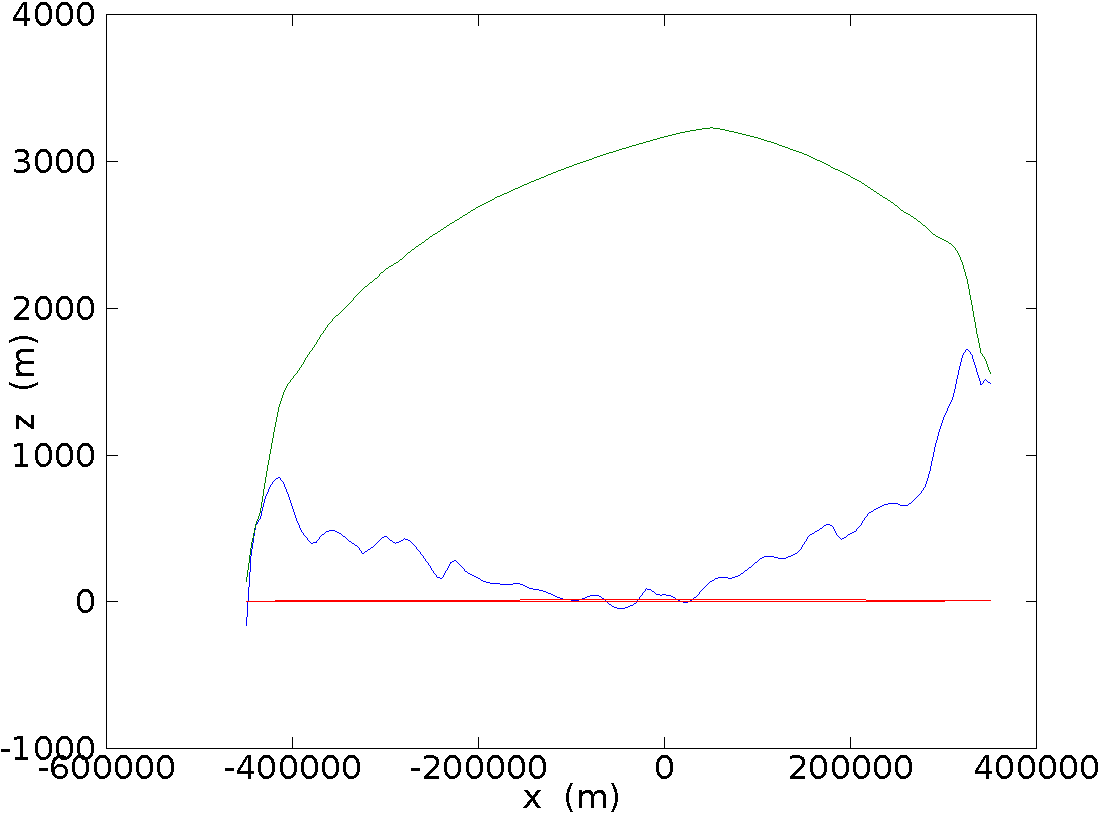
\includegraphics[width=0.5\textwidth]{greentrans}
  \end{center}
\normalsize
\item in {\color{dark red}{red}}: a view without this vertical exaggeration
\item so: numerical Stokes equations solvers require care \dots most simulations use shallow limits of Stokes
\end{itemize}
\end{frame}


\begin{frame}{deformation versus basal motion}

\begin{columns}
\begin{column}{0.35\textwidth}
\small
\begin{itemize}
\item \emph{top}:  non-sliding (SIA) and sliding/floating (SSA) modes
\item \emph{bottom}:  real transition sheet-stream-shelf (Lambert Glacier \& Amery Ice Shelf, Antarctica)
\end{itemize}
\end{column}

\begin{column}{0.65\textwidth}
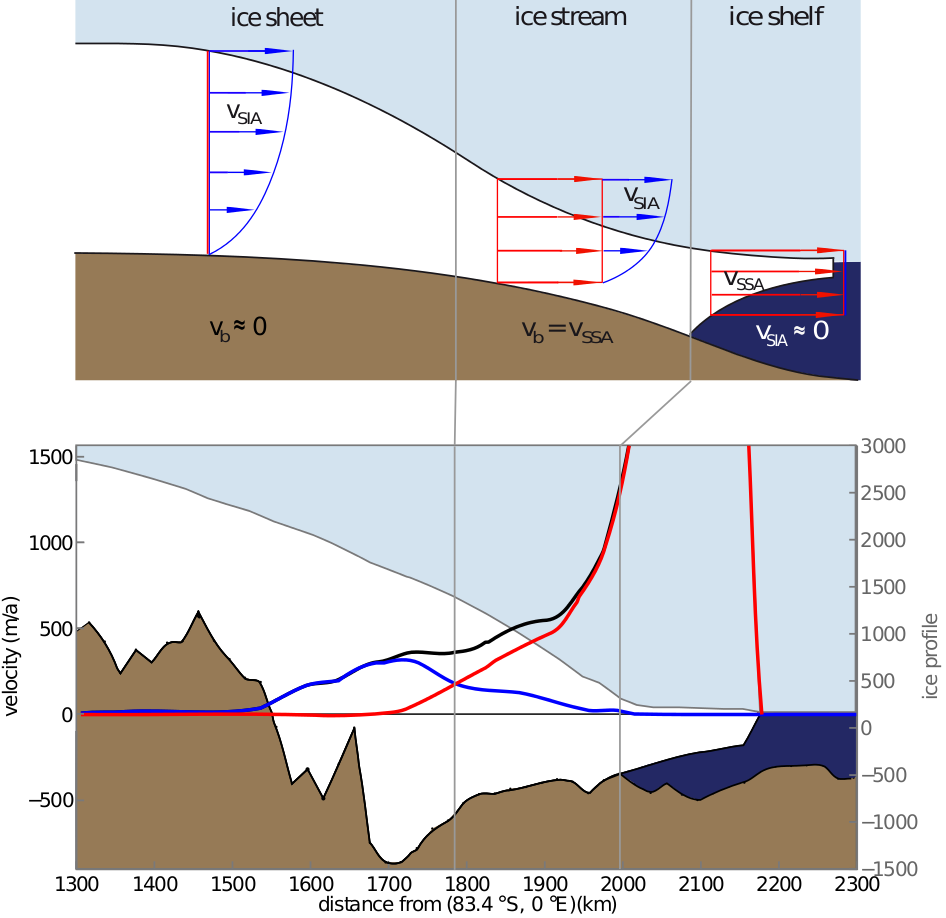
\includegraphics[width=\textwidth]{siassacartoon-lambert}
\end{column}
\end{columns}
\end{frame}


\begin{frame}{summary so far}

\begin{itemize}
\item ice sheets have four outstanding properties \emph{as viscous flows}:
  \begin{enumerate}
  \item \alert{slow}
  \item \alert{shear-thinning}
  \item \alert{shallow}
  \item \alert{contact slip}
  \end{enumerate}
\end{itemize}
\end{frame}


\begin{frame}
  \frametitle{big picture: ice sheet flow affects sea level}

\small
if we think of an ice sheet as an input/output device:
\begin{itemize}
\item \emph{inputs}: (1) snow adds, (2) sun heats, (3) earth heats
\item \emph{outputs}: (1) surface meltwater, (2) basal meltwater, (3) ice discharge
\end{itemize}

\begin{center}
  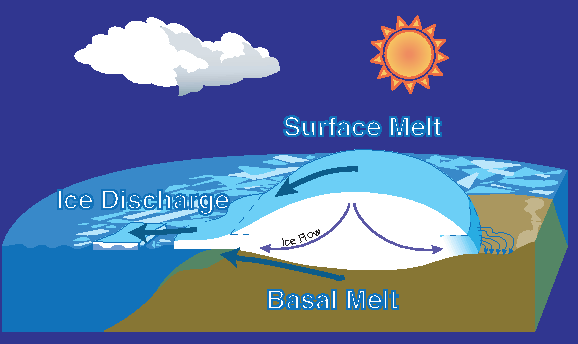
\includegraphics[width=0.7\textwidth]{ice-sheet-cartoon}

  \tiny (figure from IceSAT brochure)
\end{center}
\end{frame}


\begin{frame}
  \frametitle{big picture: ice sheet flow changes over time}

\small
\begin{itemize}
\item boxes show estimates of mass loss rate from Greenland:
\begin{center}
    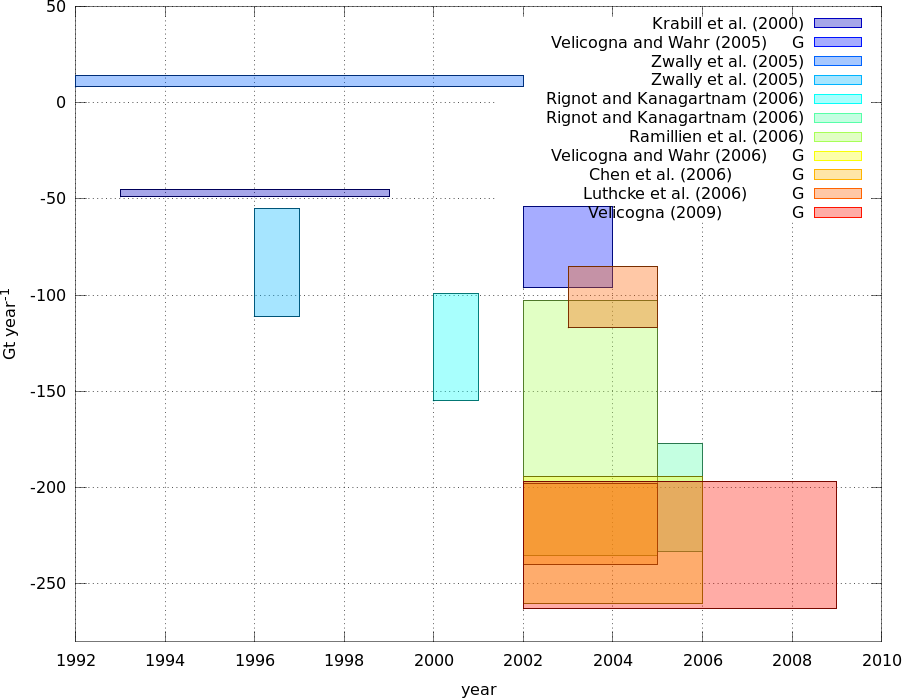
\includegraphics[width=0.55\textwidth]{greenlandboxes}
\end{center}

\vspace{-0.21in}
\item context:
  \begin{itemize}
  \item[$\circ$]  Greenland ice sheet mass is $2.7 \times 10^9$ gigatonnes (Gt $\approx \text{km}^3$) % = 2.93466 10^6 km^3  volume, from SeaRISE-Greenland 5km data
  \item[$\circ$]  if \emph{all} Greenland ice melts then we get 7 m of sea level rise
  \item[$\circ$]  if \emph{all} Antarctic ice melts then we get about 60 m of sea level rise
  \end{itemize}
\end{itemize}
\end{frame}


\section[shallow ice approximation]{shallow ice approximation for grounded ice sheets}


\begin{frame}
  \frametitle{the main variables}

\begin{center}
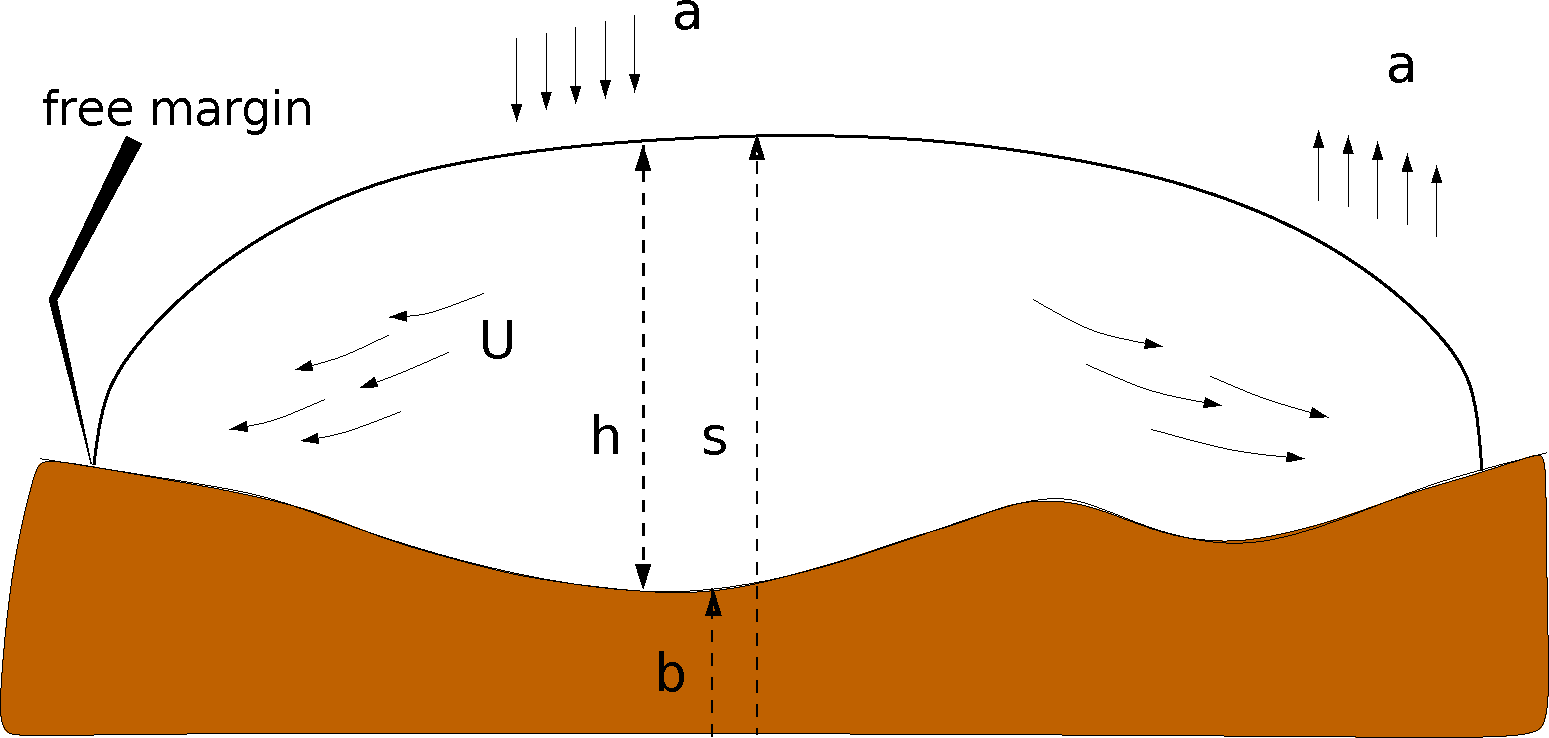
\includegraphics[width=0.7\textwidth]{groundedscheme}
\end{center}

\begin{itemize}
\item $b=b(\bx)$ the bedrock elevation
\item $s=s(\bx,t)$ the top surface elevation
\item $h=h(\bx,t)$ the ice thickness
\item ${\bf U}={\bf U}(\bx,z)$ the horizontal velocity field
\item $a=a(\bx,z)$ the yearly-average mass balance
\end{itemize}

\begin{alertblock}{key idea: \alert{ice surface is always above the bedrock}}
\end{alertblock}
\end{frame}


\begin{frame}
  \frametitle{shallow ice approximation (SIA)}

\begin{itemize}
\item SIA = lubrication approximation of Stokes flow problem
\item applies when zero or minimal sliding
\item derive SIA equations by scaling Stokes model with small parameter $\eps = [h] / [x]$ where $[h]$ is a typical thickness scale and $[x]$ is a typical width scale
\end{itemize}
\end{frame}

  
\begin{frame}
  \frametitle{shallow ice approximation: formulas}
 
\begin{itemize}
\item let $p=n+1>2$
\item assuming no sliding and isothermal ice, horizontal ice velocity ${\bf U}$ is given by: 
  $${\bf U}(\bx,z)  =  - (2A/p) (\rho_i g)^{p-1}  \left[ (s-b)^p - (s - z)^p  \right] 
|\nabla s |^{p-2} \nabla s$$
\item mass conservation (in steady state): 
  $$\Div \left(  \int_b^s {\bf U} dz \right)  =  a$$
\item shallow ice approximation + (steady) mass conservation:
  $$- \Gamma  \Div \left( (s-b)^{p+1} | \nabla s |^{p-2} \nabla s  \right) =  a(s)$$
  \begin{itemize}
  \vspace{-0.2in}
  \item[$\circ$] which is the major SIA equation \dots a PDE?
  \item[$\circ$] generalizes $p$-Laplace equation $\Div \left( | \nabla u |^{p-2} \nabla u  \right) =  0$
  \end{itemize}
\end{itemize}
\end{frame}


\begin{frame}
  \frametitle{a change of variable}
 
\begin{itemize}
\item using the change of variable  $u=(s-b)^{ \frac{2p}{p-1}}$, we obtain a revised $p$-Laplace equation
\begin{equation*}
 -  \Div \left( \mu  | \nabla u - \Phi(u) |^{p-2}
  ( \nabla u - \Phi(u) )  \right)  = \alpha(u)
\end{equation*}
where
  \begin{itemize}
  \item[$\circ$]  $\Phi(u) = - C \, u^{\frac{p+1}{2p}} \nabla b(\bx)$ is a transformed bedrock topography which ``tilts'' the $p$
  \item[$\circ$]  $\alpha(u) = a(\bx,u^{\frac{p-1}{2p}} )$ is transformed mass balance (source term)
  \end{itemize}
and $\mu>0$ is constant (in the isothermal case)
\end{itemize}
\end{frame}


\begin{frame}
  \frametitle{ variational inequality } 

\begin{itemize}
\item $u=(s-b)^{ \frac{2p}{p-1}}$ is a power of the \emph{thickness} $h=s-b$
\item thickness is nonnegative!
\item the change $s \to u$ transforms the constraint $s \ge b$ into $u \ge 0$
\item previous PDE applies only when $u>0$
\item to get a weak formulation we integrate-by-parts as usual
\end{itemize}

\begin{block}{Definition} 
A function $u \in \Kcal := \{ v \in W^{1,p}_0 (\Omega), v \ge 0 \}$ 
solves the (transformed) steady shallow ice sheet problem if
\begin{align*}
\int_{\Omega}    \left( \mu  | \nabla u - \Phi(u) |^{p-2} 
( \nabla u - \Phi(u) )    \right)  \cdot \nabla ( v - u )  
\ge \int_{\Omega} \alpha(u) (  v -  u ) 
\end{align*}
for all $v \in \Kcal$.
\end{block}
\end{frame}


\begin{frame}
  \frametitle{shallow ice approximation (SIA): an analogy}

\begin{columns}
\begin{column}{0.35\textwidth}
\begin{itemize}
\item ice sheet surface \\ = \alert{membrane}
\item bedrock = \alert{obstacle}
\end{itemize}
\vfill
\begin{center}
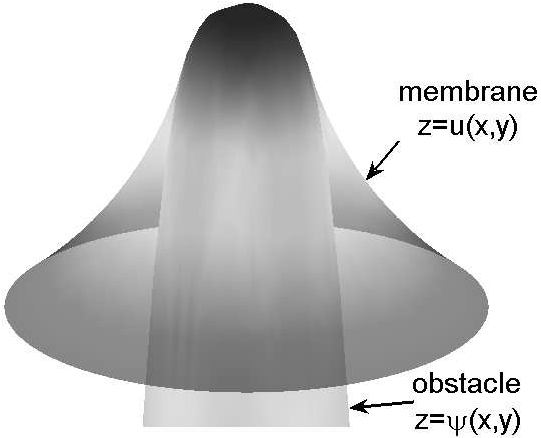
\includegraphics[width=1.1\textwidth]{classicalobs}
\end{center}
\end{column}
\begin{column}{0.65\textwidth}
\begin{center}
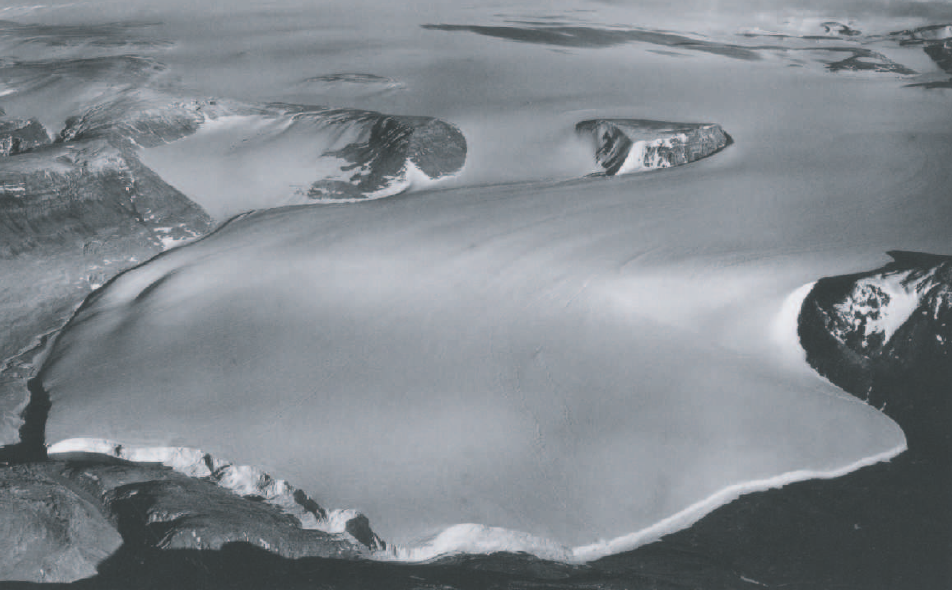
\includegraphics[width=0.8\textwidth]{polaris} \\
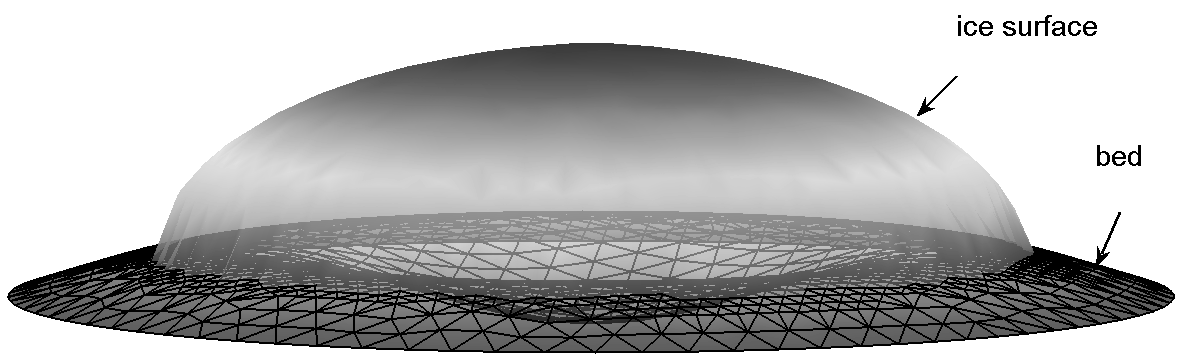
\includegraphics[width=\textwidth]{capnonflatobs}
\end{center}
\end{column}
\end{columns}
\end{frame}


\frame{  \frametitle{ Existence and uniqueness of solutions } 

 \onslide<+-> 

\begin{block}{Convex minimization}
If $a$ is independent of $u$, the variational inequality rewrites:
\begin{equation*}
J(u) = \min_{v \in \Kcal} \left\{  J(v):= \frac{\mu}{p} \int_{\Omega} 
 |\nabla v - \Phi |^p - \int_{\Omega}  \alpha v \right\} 
\end{equation*}
which admits a unique solution.
\end{block}

 \onslide<+->

\hfill $ \Rightarrow $ Existence and uniqueness only if the bedrock is flat ($\Phi = 0$). \\

 \onslide<+->
 
\begin{block}{Monotone operator}
If $a$ is not increasing with respect to $u$, 
we still have a unique solution by monotonicity of 
\begin{center}
$(Av)(w)= \mu \int_{\Omega} | \nabla v - \Phi|^{p-2} ( \nabla v  - \Phi )
\cdot \nabla w - \int_{\Omega}  \alpha(v) w .$
\end{center}
\end{block}
}
 
 
\frame{  \frametitle{ Existence in the general case } 

 \onslide<+->

Define the map $\mathcal{A}:C(\overline{\Omega}) \rightarrow C(\overline{\Omega})$,
which takes $w$ to the unique $u$ solving, for all $v \in \mathcal{K}$:
\begin{align*}
\int_{\Omega}   \mu  \left( | \nabla u - \Phi(w) |^{p-2} 
( \nabla u - \Phi(w) )    \right)  \cdot \nabla ( v - u )  
\ge \int_{\Omega} \alpha(w) (  v -  u ),
\end{align*} 

\begin{block}{Result}
If $p>2$, the map $\mathcal{A}$ admits at least one fixed point.
\end{block}

  \onslide<+->
  
\begin{block}{Idea of the proof}
\begin{itemize}
\item $\mathcal{A}$ is continuous and compact.
\item $\{ w \in C(\overline{\Omega}), \; \exists \lambda \in [0,1] , 
\, \quad w = \lambda \mathcal{A}(w)   \}$ is bounded. 
\item Conclude with Schaefer's fixed point theorem.
\end{itemize}
\end{block}
 
} 


\frame{  \frametitle{ In the most general case  } 

\onslide<+->
If we include the temperature dependence and the basal sliding, 
ice velocity ${\bf U}$ is given by:

\begin{equation*}
{\bf U}(\bx,z)  = \underbrace{ -2 (\rho_i g)^{p-1} 
\left[ \int_b^z A(\bx,s)(s-t)^{p-1} dt \right] 
|\nabla s |^{p-2} \nabla s}_{\text{Ice shearing}} +   
\underbrace{{\bf U}_b}_{\text{Basal sliding}}, 
\end{equation*}

\onslide<+->

and the mass conservation equation rewrites: 

\begin{equation*}
 -  \Div \left( \mu(u) | \nabla u - \Phi(u) |^{p-2} 
  ( \nabla u - \Phi(u) ) - \Psi (u)  \right)  = \alpha(u), 
\end{equation*}   
where 
\begin{align*}
 \mu(u)  = C  \int_0^1 A(\bx,  b + t u^{\frac{p-1}{2p}}) ( 1 - t )^p dt, 
 \quad {\rm and} \quad 
 \Psi(u)  = u^{\frac{p-1}{2p}} \, {\bf U}_b(\bx). 
\end{align*}

\onslide<+->

The variational inequality rewrites 
\begin{align*}
\int_{\Omega}    \left( \mu(u)  | \nabla u - \Phi(u) |^{p-2} 
( \nabla u - \Phi(u) )  - \Psi (u )  \right)  \cdot \nabla ( v - u )
\ge \int_{\Omega} \alpha(u) (  v -  u ). 
\end{align*} 

\onslide<+->

Existence can be extended but uniqueness issues remain open.
}


\begin{frame}
  \frametitle{steady ice sheet over Greenland bedrock }

\small
Given: $a$ and $b$.  Set $u_0 = 0$.  Do fixed point iterations ($i=0,1,2,3$):
$$  \int_{\Omega}    \left( \mu  | \nabla u_{i+1} - \Phi(u_i) |^{p-2}
( \nabla u_{i+1} - \Phi(u_i) )    \right)  \cdot \nabla ( v - u_{i+1} )
\ge \int_{\Omega} \alpha (  v -  u_{i+1} ).$$

\begin{center}
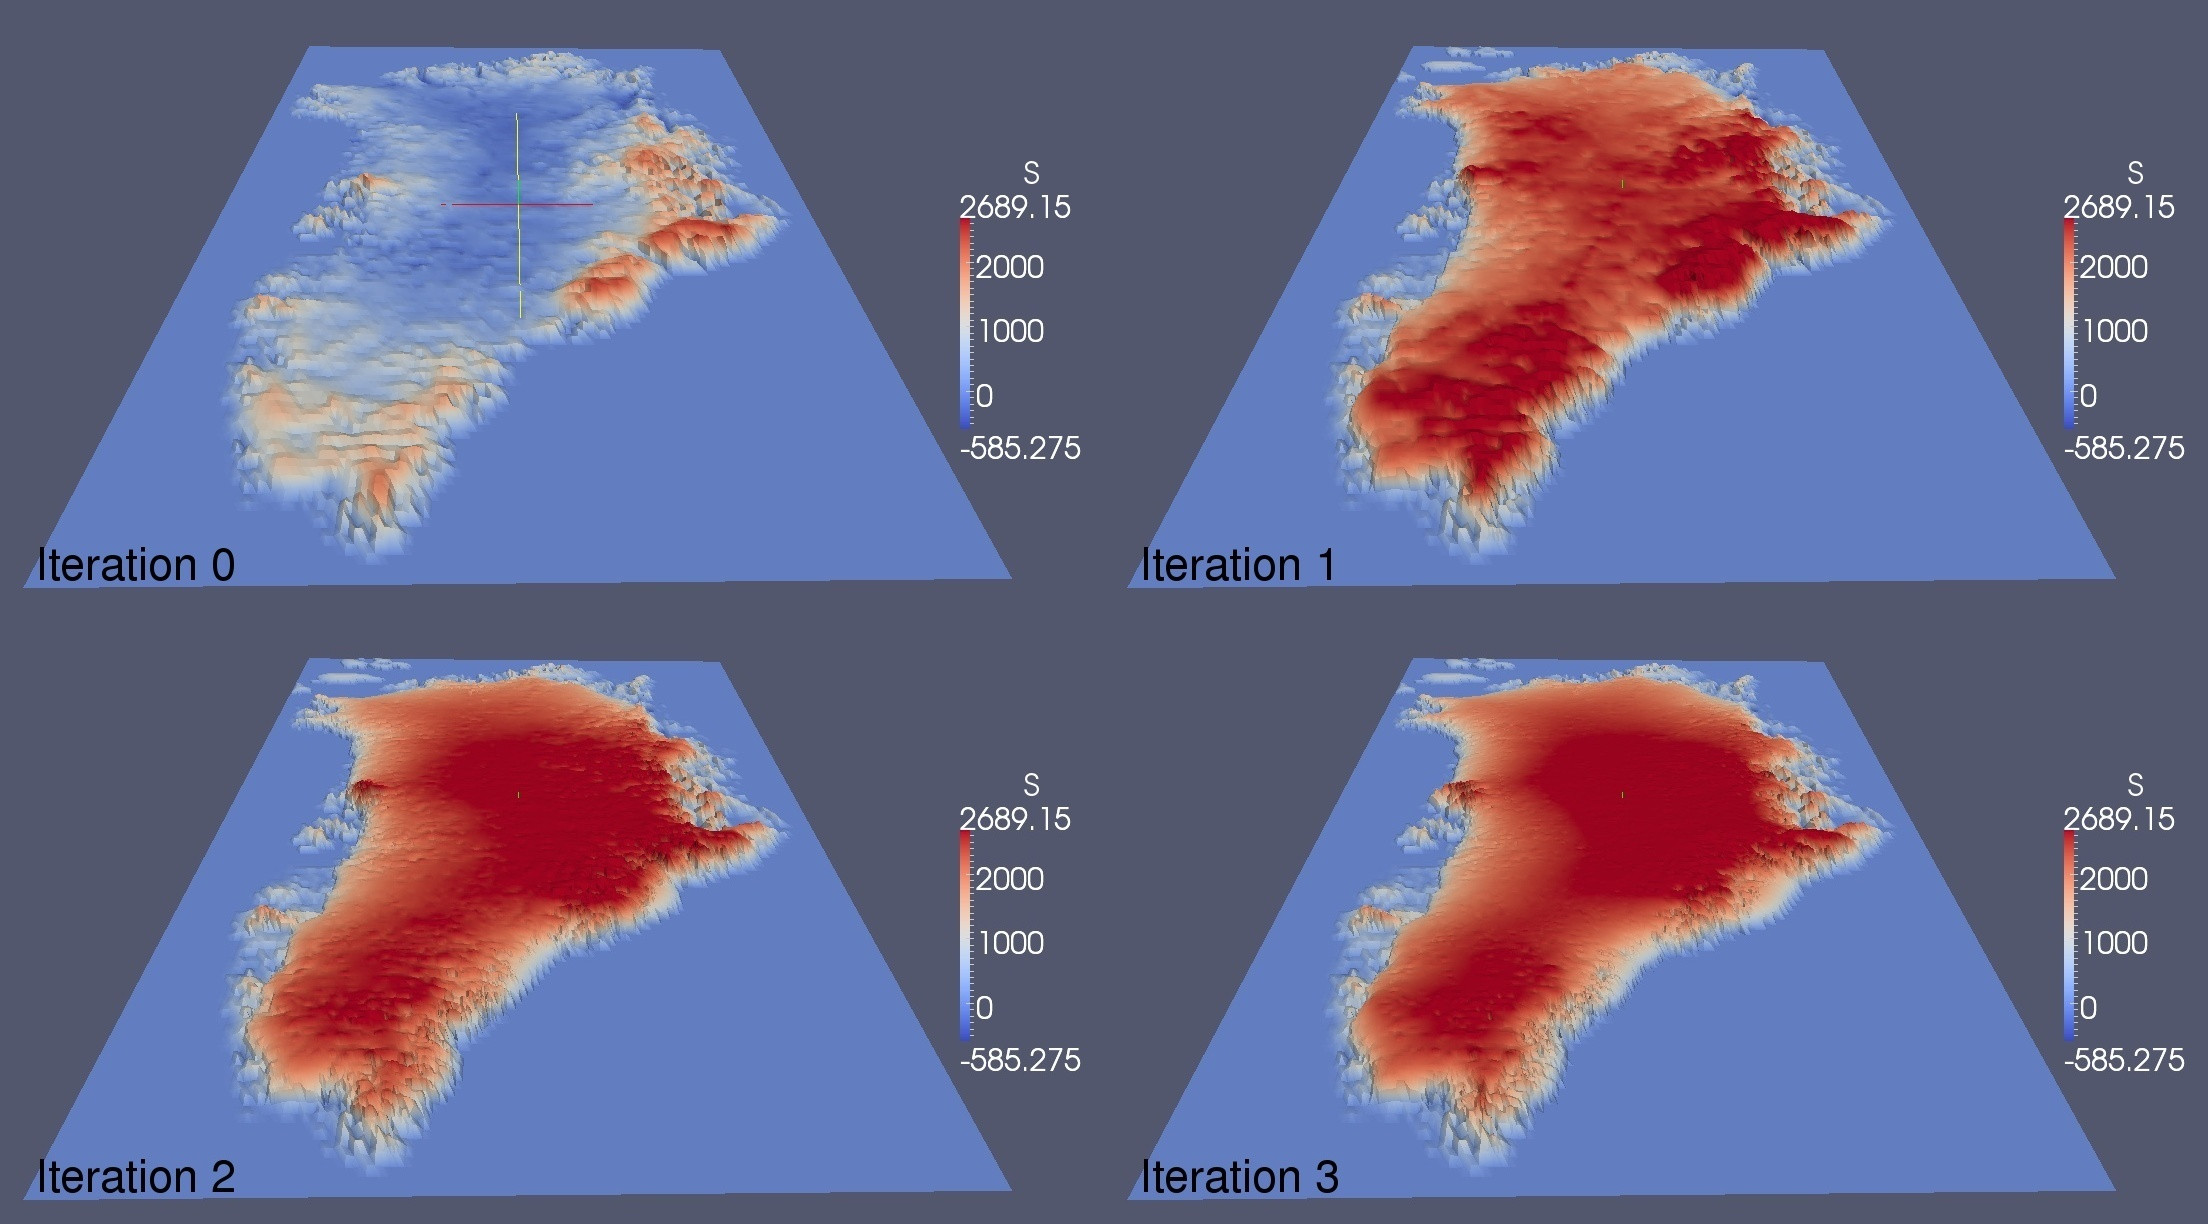
\includegraphics[width=0.9\textwidth]{greenland-result.jpg}
\end{center}
\end{frame}


\section[ice streams]{a model for ice streaming}


\begin{frame}
  \frametitle{shallow shelf approximation (SSA): a definition}

\begin{itemize}
\item FIXME
\end{itemize}
\end{frame}


\begin{frame}
  \frametitle{shallow shelf approximation (SIA): an analogy}

\begin{itemize}
\item FIXME: schoof's sliders picture
\end{itemize}
\end{frame}


\section[marine ice sheets]{a model for marine ice sheet evolution}

\begin{frame}
  \frametitle{moving grounding line}

FIXME: model is SIA+SSA with adaptive grid

\begin{center}
\PDFAnimation{exp3a}
\end{center}
\end{frame}


\section[polythermal ice]{awaiting a weak formulation: polythermal ice}

\section*{conclusion}

\begin{frame}
  \frametitle{conclusion: some new thinking which is weak and shallow}

\begin{itemize}
\item work on steady states (walk before fly)
\item steady grounded ice sheets now have a well-posed obstacle-like formulation (a $p>2$-Laplace variational inequality for SIA+mass)
\item sliding ice sheets have a theory in which ice streams ``emerge naturally'' (a $p<2$-Laplace variational inequality for SSA)
\item marine ice sheet paradigm from time-splitting:
  \begin{itemize}
  \item[$\circ$]  solve SSA problem
  \item[$\circ$]  advection with SSA velocity
  \item[$\circ$]  solve SIA+mass obstacle problem
  \end{itemize}
\end{itemize}
\end{frame}


%%%%%%%%%%%%%%


\section*{extra slides}

\begin{frame}
  \frametitle{full and simplified (shallow) ice flow models }

\begin{center}
\begin{tabular}{|c|c|c|}
\hline name & unknowns  & equation (+incompressibility)   \\ 
\hline Stokes & 
$\left(
\begin{array}{c}
u \\ 
v \\ 
w  
\end{array} \right),p$ &  
$  \nabla \cdot \left(
\begin{array}{ccc}
\tau_{xx} & \tau_{xy} & \tau_{xz} \\ 
\tau_{yx} & \tau_{yy} & \tau_{yz} \\ 
\tau_{zx} & \tau_{zy} & \tau_{zz}  
\end{array} \right) = \left(
\begin{array}{c}
0 \\ 
0 \\ 
\rho g  
\end{array} \right)$  \\ 
\hline B.-P.\footnote{\tiny Blatter-Pattyn approximation} & 
$\left(
\begin{array}{c}
u \\ 
v 
\end{array} \right) $  & 
$ \nabla \cdot \left(
\begin{array}{ccc}
\tau_{xx} & \tau_{xy} & \tau_{xz} \\ 
\tau_{yx} & \tau_{yy} & \tau_{yz} \\ 
0 & 0 & \tau_{zz}  
\end{array} \right) = \left(
\begin{array}{c}
0 \\ 
0 \\ 
\rho g  
\end{array} \right)$  \\  
\hline SSA\footnote{\tiny shallow shelf approximation} &
$ \left(
\begin{array}{c}
u \\ 
v  
\end{array} \right) $ & 
$ \nabla \cdot \left(
\begin{array}{ccc}
\tau_{xx} & \tau_{xy} & 0 \\ 
\tau_{yx} & \tau_{yy} & 0 \\ 
0 & 0 & \tau_{zz}  
\end{array} \right) = \left(
\begin{array}{c}
0 \\ 
0 \\ 
\rho g  
\end{array} \right)$ \\ 
\hline SIA\footnote{\tiny shallow ice approximation} & $\emptyset$ &
$ \nabla \cdot \left(
\begin{array}{ccc}
0 & 0 & \tau_{xz} \\ 
0 & 0 & \tau_{yz} \\ 
0 & 0 & \tau_{zz}  
\end{array} \right) = \left(
\begin{array}{c}
\rho g \frac{\partial s}{\partial x}\\ 
\rho g \frac{\partial s}{\partial y} \\ 
\rho g  
\end{array} \right)$ \\ 
\hline 
\end{tabular}  
\end{center}
  
\end{frame}


\end{document}

